\documentclass[tikz,border=1pt]{standalone}
\usepackage{pgfplots}
\pgfplotsset{compat=1.18}
\begin{document}
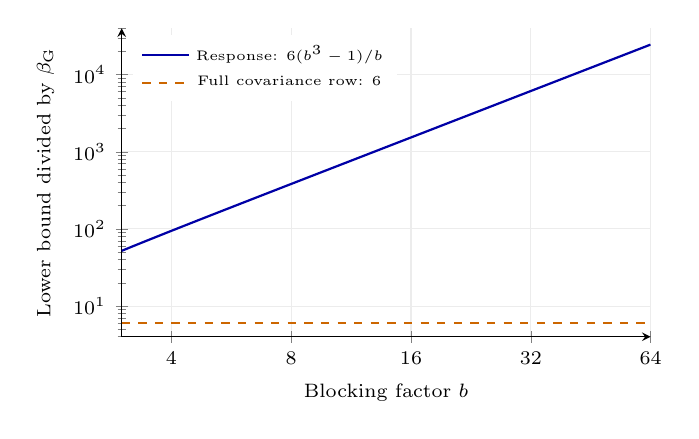
\begin{tikzpicture}
\begin{axis}[width=8.3cm,height=5.5cm,xmode=log,ymode=log,
 xmin=3,xmax=64,ymin=4,ymax=40000,
 xlabel={Blocking factor $b$},ylabel={Lower bound divided by $\beta_{\rm G}$},
 xtick={4,8,16,32,64},xticklabels={4,8,16,32,64},
 tick label style={font=\scriptsize},label style={font=\scriptsize},
 grid=major,grid style={gray!15},axis lines=left,
 legend style={font=\tiny,draw=none,at={(.02,.98)},anchor=north west}]
\addplot[blue!65!black,thick,domain=3:64,samples=100]{6*(x^3-1)/x};
\addlegendentry{Response: $6(b^3-1)/b$}
\addplot[orange!80!black,dashed,thick,domain=3:64]{6};
\addlegendentry{Full covariance row: $6$}
\end{axis}
\end{tikzpicture}
\end{document}
